\newpage
\section*{APPENDICES} 
\phantomsection
\addcontentsline{toc}{section}{APPENDICES}

% ===== Appendix A =====
\subsection*{Appendix A: Project Budget}
\phantomsection
\addcontentsline{toc}{subsection}{Appendix A: Project Budget}

\label{app:budget}
\renewcommand{\thetable}{A-\arabic{table}}
\setcounter{table}{0} 
\begin{table}[H]
\centering
\caption{Project Budget Expenses}
\label{tab:budget-estimation}
\renewcommand{\arraystretch}{1.4} 
\begin{tabularx}{\textwidth}{|l|>{\raggedleft\arraybackslash}X|>{\raggedleft\arraybackslash}X|>{\raggedleft\arraybackslash}X|}
\hline
\textbf{Item} & \textbf{Quantity} & \textbf{Rate (NRs.)} & \textbf{Total (NRs.)} \\
\hline
ESP32-S3 DevKit & 2 & 1600 & 3200 \\
\hline
NEMA 17 Stepper Motor & 1 & 1250 & 1250 \\
\hline
MG996R Servo Motor & 1 & 800 & 800 \\
\hline
Bulb Holder Pin & 6 & 30 & 180 \\
\hline
A4988 Motor Driver & 2 & 200 & 400 \\
\hline
100 $\mu$F Capacitor & 5 & 20 & 100 \\
\hline
18650 Li-Ion Battery & 6 & 500 & 3000 \\
\hline
3S 18650 Battery Holder & 1 & 150 & 150 \\
\hline
3S 20A BMS Board & 1 & 350 & 350 \\
\hline
LM2596 Buck Converter & 1 & 600 & 600 \\
\hline
2.4 GHz Directional Antenna & 2 & 1200 & 2400 \\
\hline
SMA Pigtail Cable & 2 & 500 & 1000 \\
\hline
Coupler & 1 & 200 & 200 \\
\hline
Logistics and Miscellaneous & -- & -- & 3000 \\
\hline
\multicolumn{3}{|l|}{\textbf{Total Cost}} & \textbf{16,630} \\
\hline
\end{tabularx}
\end{table}

\newpage
\subsection*{Appendix B: Gantt Chart}
\phantomsection
\addcontentsline{toc}{subsection}{Appendix B: Gantt Chart}

\label{app:gantt_char}
\renewcommand{\thetable}{B-\arabic{table}}
\setcounter{table}{0} 

\begin{table}[H]
\centering
\caption{Project Timeline}
\label{tab:gantt_char}

% Include image without nesting figure
\includegraphics[width=1\textwidth]{images/gantt_chart.png}

\end{table}

\newpage
\subsection*{Appendix C: Hardware Design}
\phantomsection
\addcontentsline{toc}{subsection}{Appendix C: Hardware Design}

\vspace{1.5em}
\renewcommand{\thefigure}{C-\arabic{figure}}
\setcounter{figure}{0} 


\begin{figure}[H]
\centering
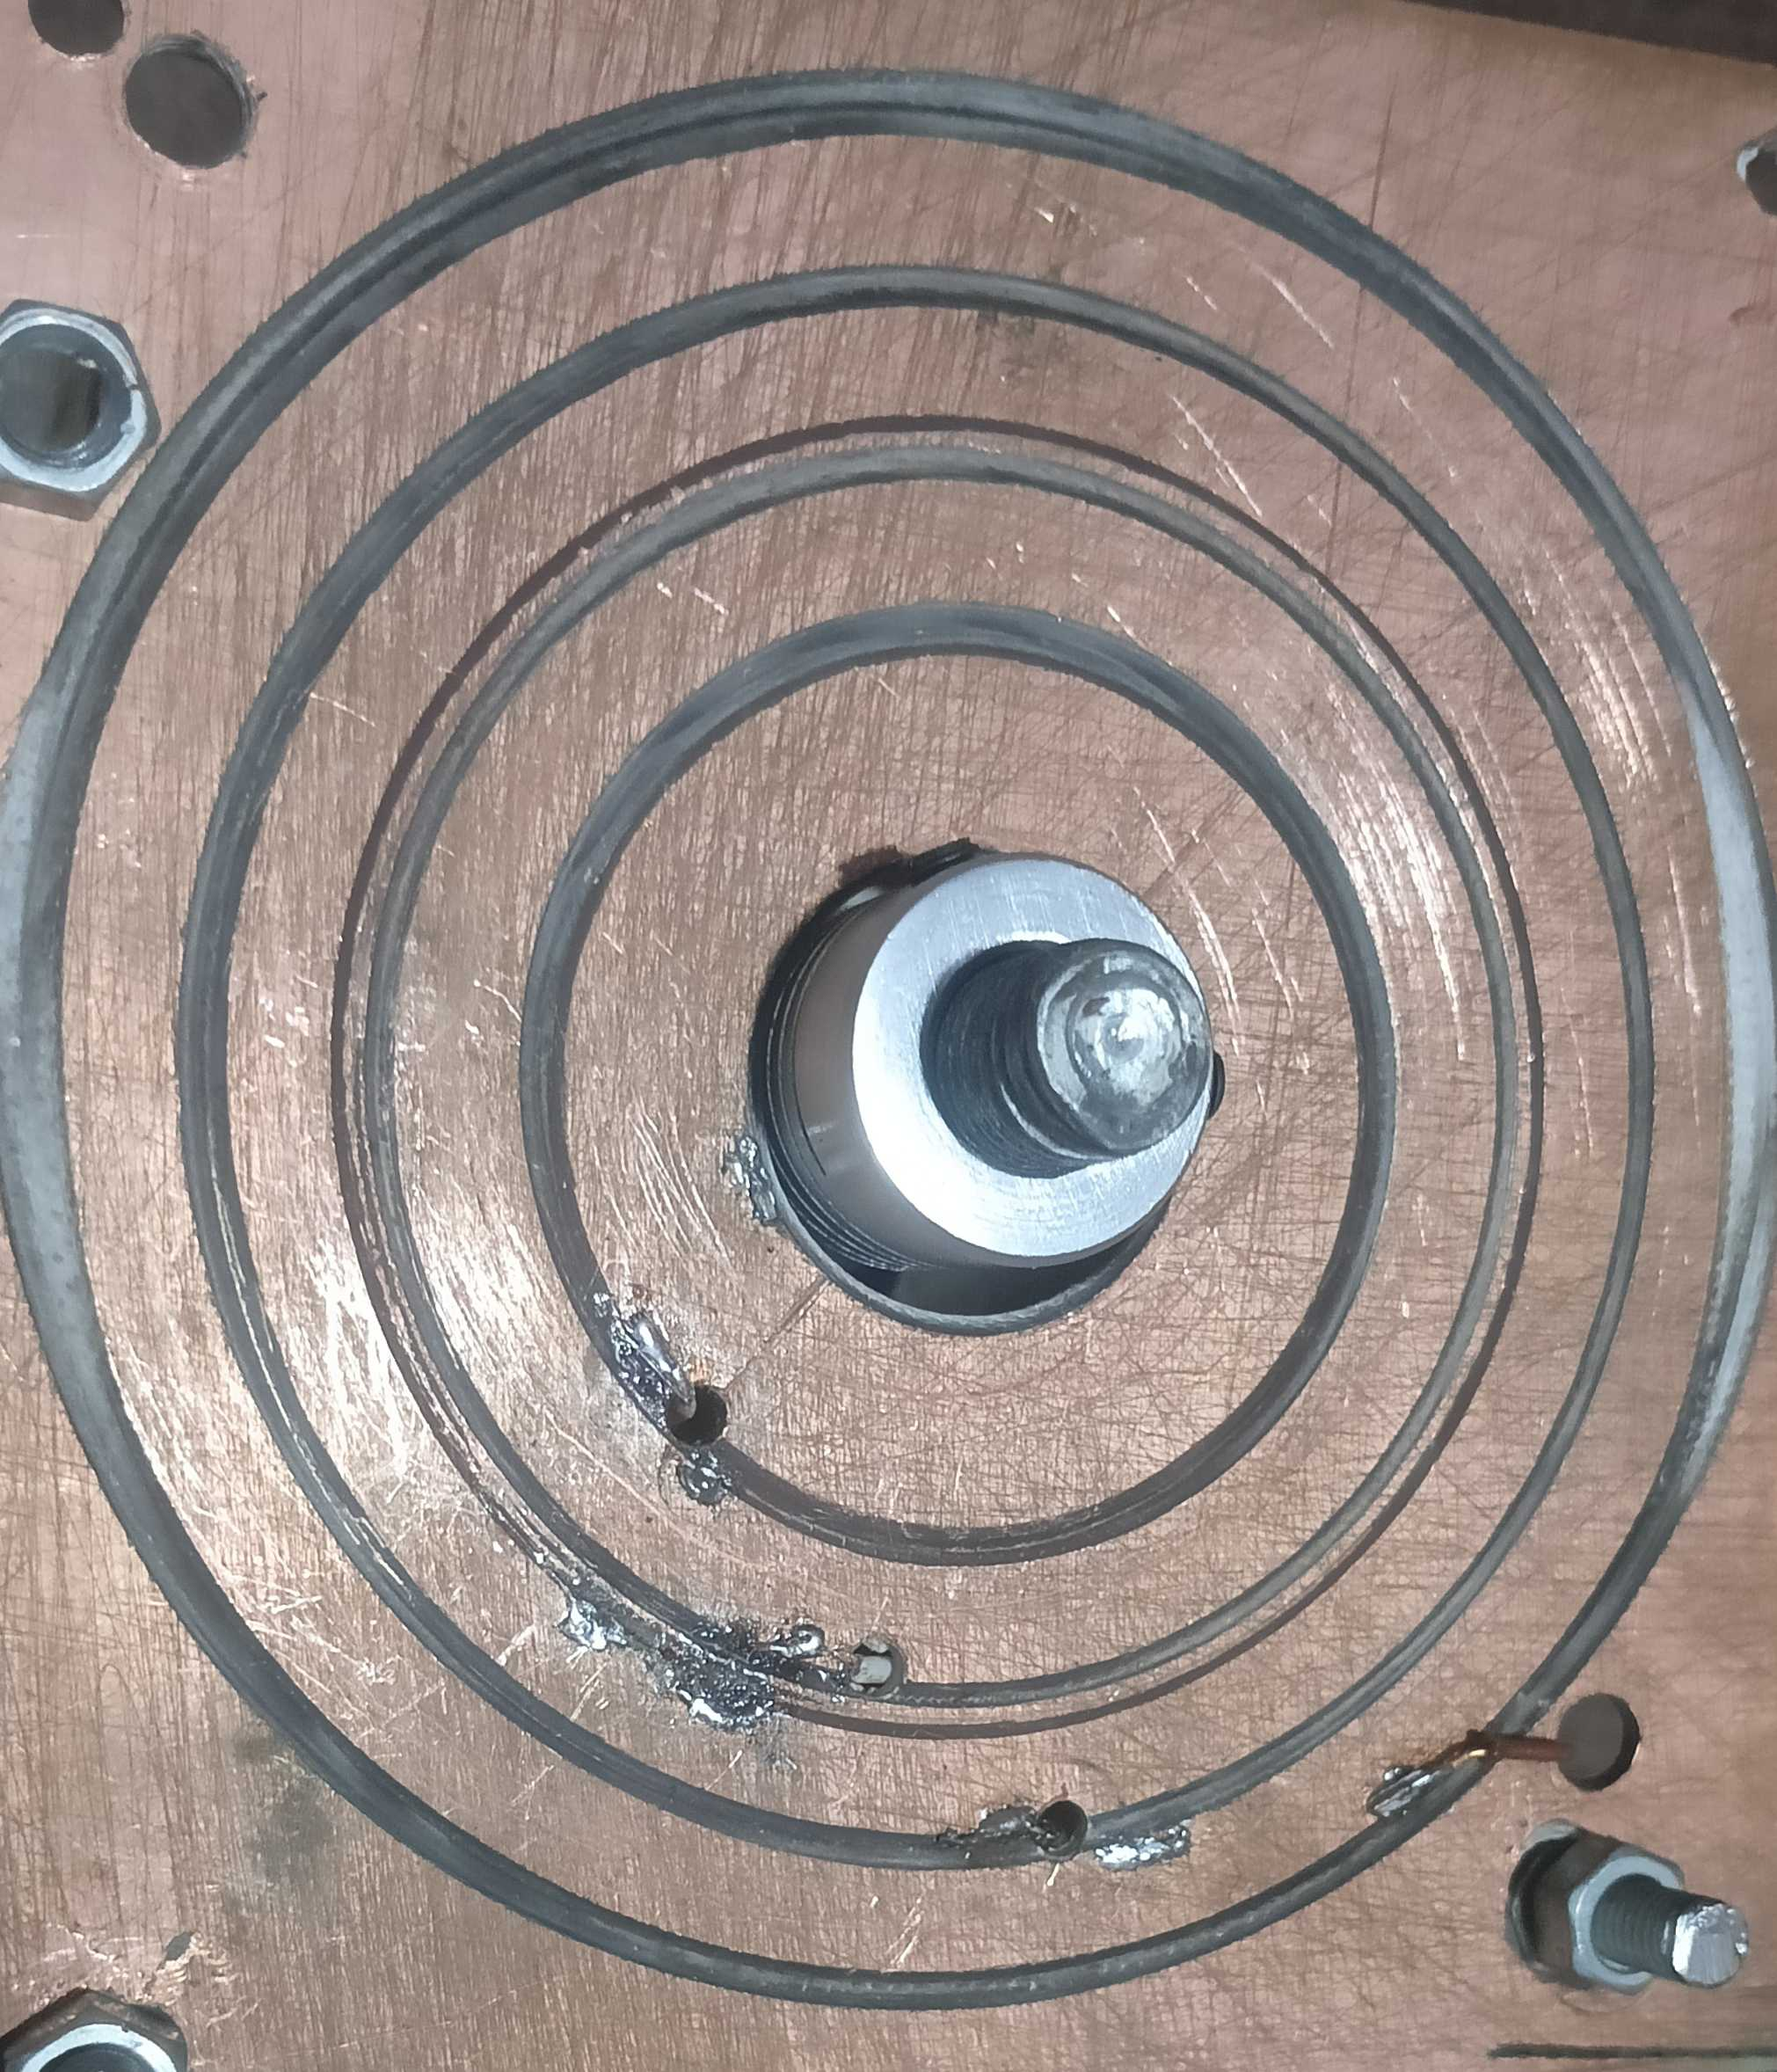
\includegraphics[width=0.6\textwidth]{images/slip_ring.png}
\caption{Design of Copper Slip Ring}
\label{fig:slip_ring}
\end{figure}


\begin{figure}[H]
\centering
\includegraphics[width=0.6\textwidth]{images/hardware_conn.png}
\caption{Connection of Mechanical Parts and Devices}
\label{fig:hardware_imp}
\end{figure}


\newpage
\subsection*{Appendix D: PCB Design}
\phantomsection
\addcontentsline{toc}{subsection}{Appendix D: PCB Design}

\vspace{1.5em}
\renewcommand{\thefigure}{D-\arabic{figure}}
\setcounter{figure}{0} 

\begin{figure}[H]
\centering
\includegraphics[width=0.8\textwidth]{images/pcb_design.png}
\caption{Footprint of PCB Design}
\label{fig:schematic_pcb}
\end{figure}


\begin{figure}[H]
\centering
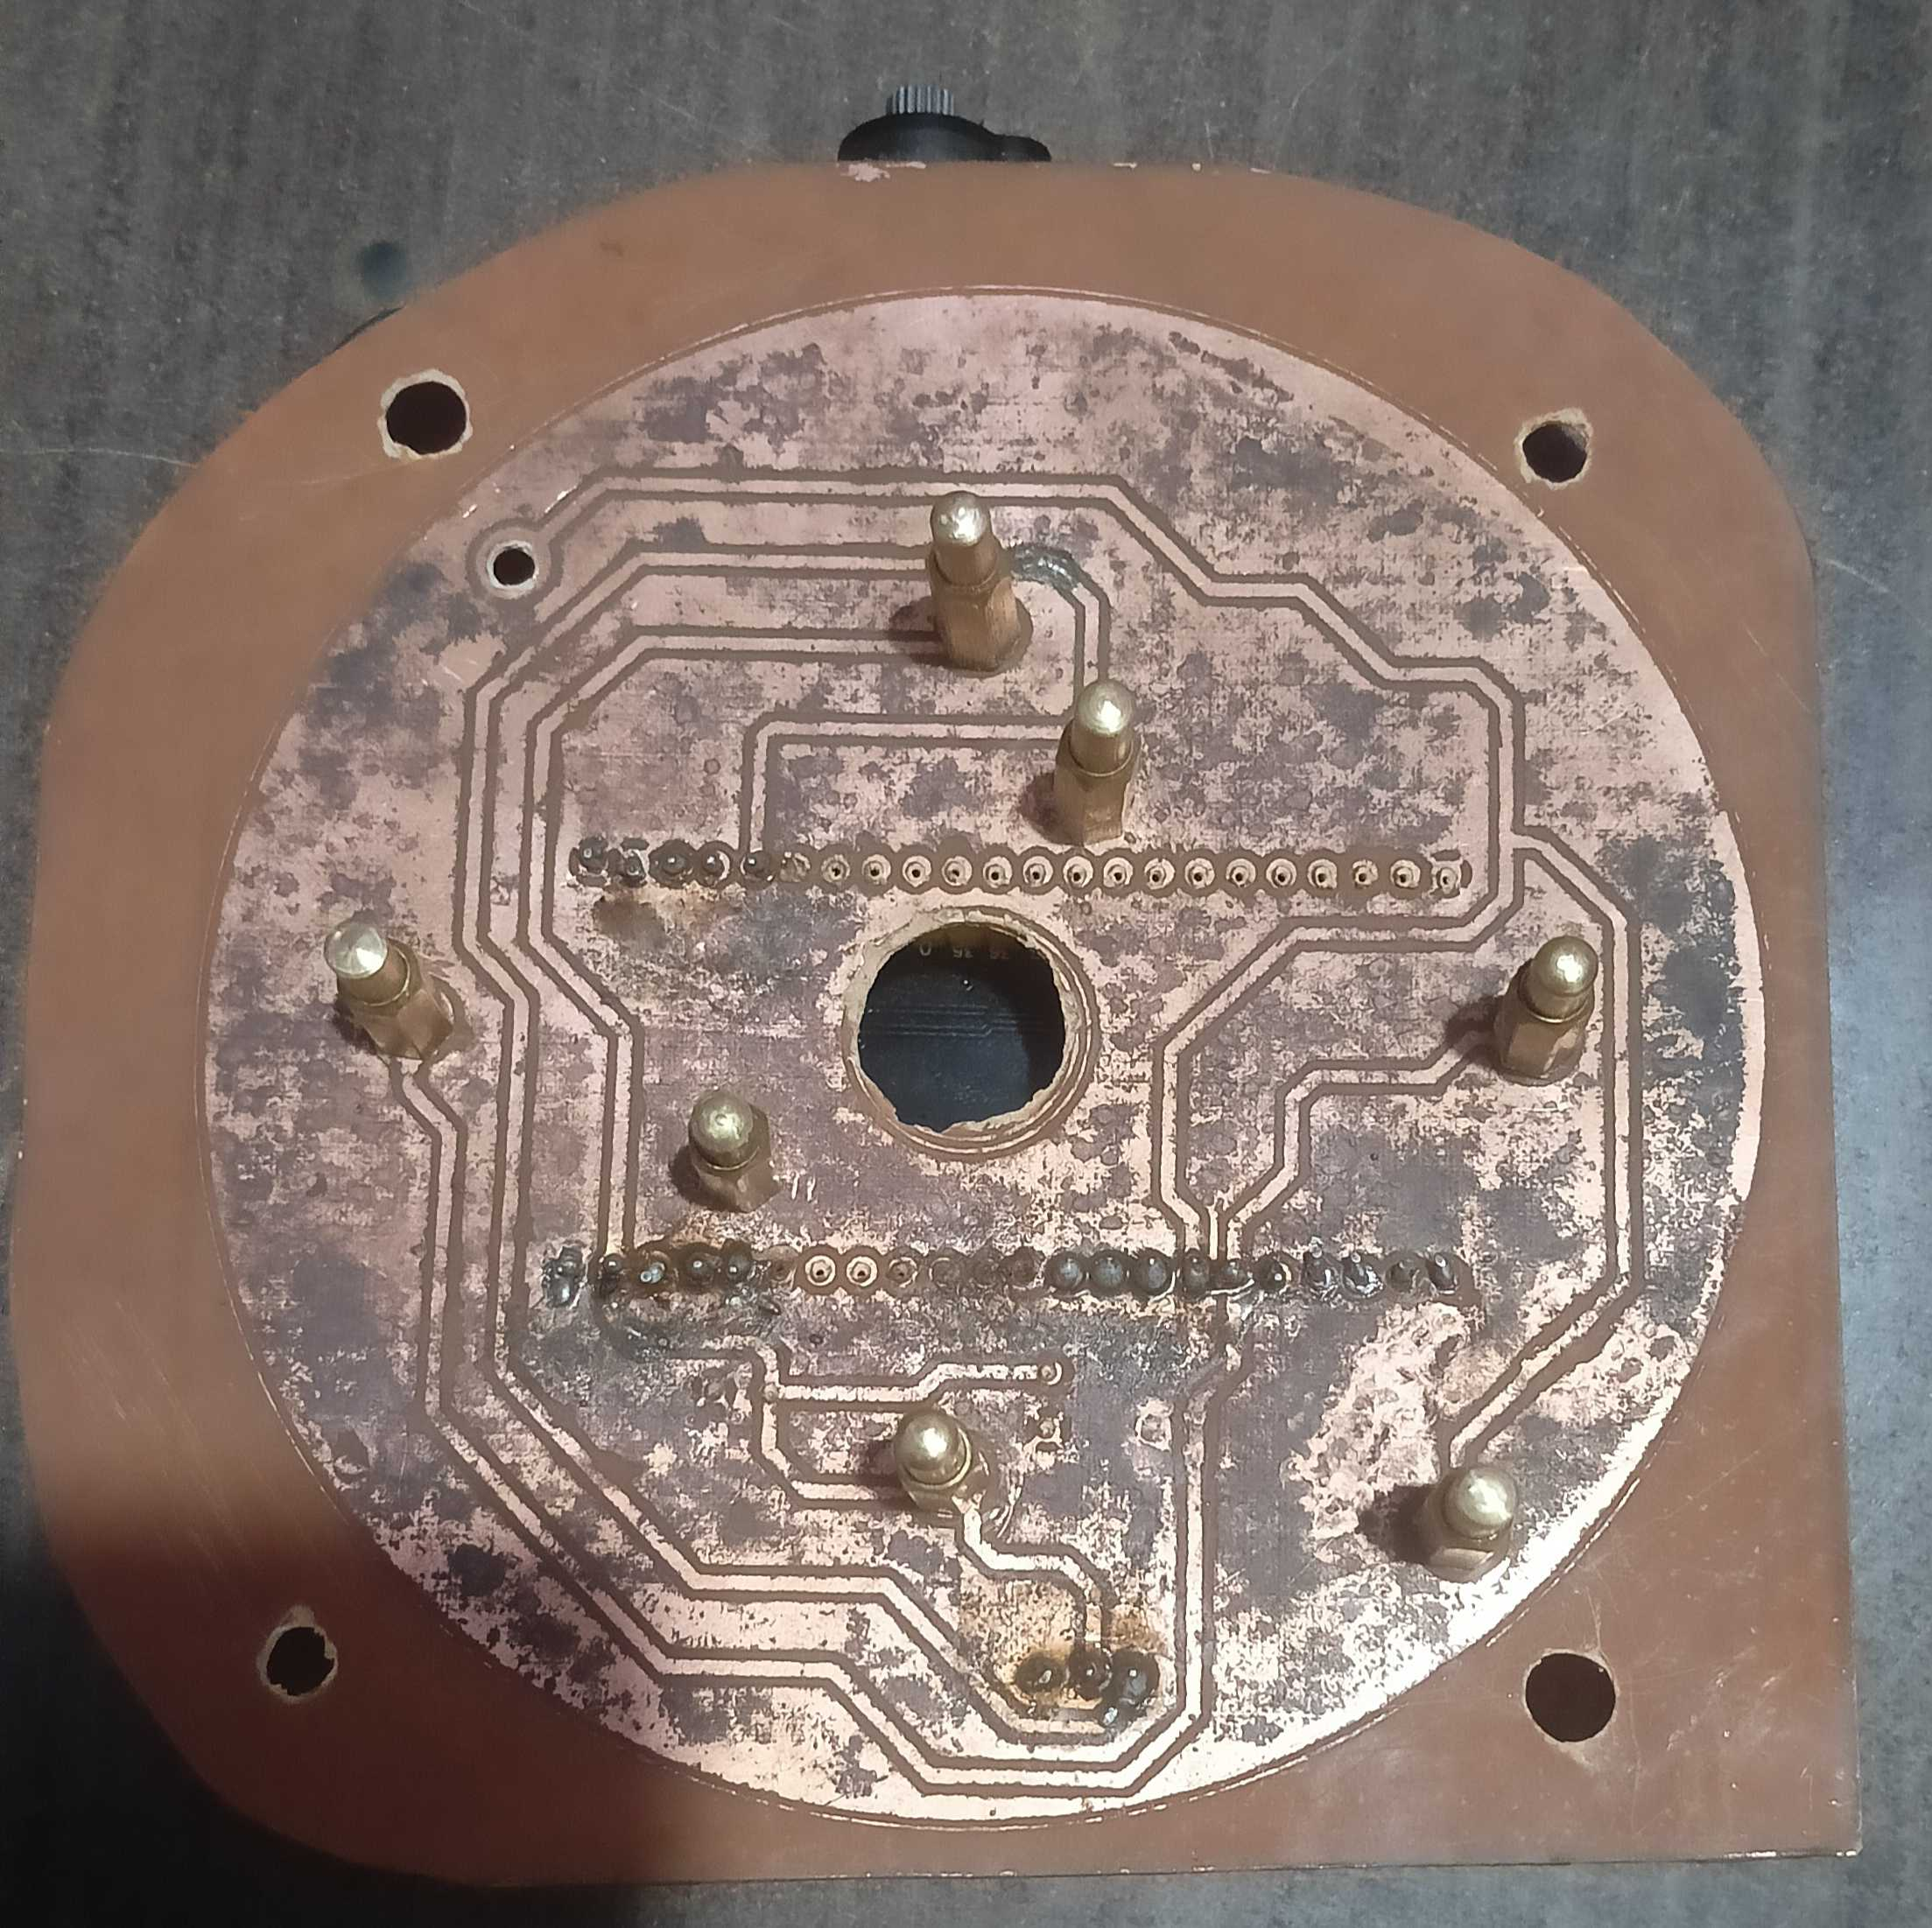
\includegraphics[width=0.7\textwidth]{images/pcb_imp.png}
\caption{PCB Design}
\label{fig:pcb}
\end{figure}


\newpage
\subsection*{Appendix E: Code Snippets}
\phantomsection
\addcontentsline{toc}{subsection}{Appendix E: Code Snippets}

\subsubsection*{Q-learning Trainer Class}
\phantomsection
\addcontentsline{toc}{subsubsection}{Q-learning Trainer Class}
\begin{minted}[linenos, fontsize=\small]{python}
class QLearningTrainer(RLAgentBase):
    ...
    # Internal safety
    def _check_state(self, s: Tuple[int, int, int]):
        p, t, d = s
        if not (0 <= p < self.pan_states):
            raise ValueError(f"Pan index out of range: {p}")
        if not (0 <= t < self.tilt_states):
            raise ValueError(f"Tilt index out of range: {t}")
        if not (0 <= d < self.delta_states):
            raise ValueError(f"Delta index out of range: {d}")

    # Action selection (ε-greedy with tie-breaking)
    def select_action(self, state: Tuple[int, int, int]) -> int:
        self._check_state(state)
        p, t, d = state

        # exploration
        if np.random.rand() < self.epsilon:
            return np.random.randint(self.n_actions)

        # greedy with random tie-breaking
        q = self.Q[p, t, d]
        max_q = np.max(q)
        best_actions = np.flatnonzero(q == max_q)

        return int(np.random.choice(best_actions))

    # Q-learning update
    def update(
        self,
        state: Tuple[int, int, int],
        action: int,
        reward: float,
        next_state: Tuple[int, int, int],
    ):
        self._check_state(state)
        self._check_state(next_state)

        p, t, d = state
        pn, tn, dn = next_state

        best_next = np.max(self.Q[pn, tn, dn])
        td_target = reward + self.gamma * best_next
        td_error = td_target - self.Q[p, t, d, action]

        self.Q[p, t, d, action] += self.alpha * td_error

        # clip for numerical stability
        self.Q[p, t, d, action] = np.clip(
            self.Q[p, t, d, action],
            self.q_clip[0],
            self.q_clip[1],
        )
    ...

\end{minted}

\subsubsection*{RL Environment Class}
\phantomsection
\addcontentsline{toc}{subsubsection}{RL Environment Class}
\begin{minted}[linenos, fontsize=\small]{python}
class RLEnvironment(RLEnvironmentBase):
    ...
    def step(self, action_id):
        axis, direction = RLConfig.ACTIONS[action_id]

        # - apply action--
        if axis == "PAN":
            self.pan += direction * RLConfig.STEP_DEG
        elif axis == "TILT":
            self.tilt += direction * RLConfig.STEP_DEG
        elif axis == "STAY":
            pass

        # enforce mechanical limits
        self.pan = int(np.clip(self.pan, 
        RLConfig.PAN_MIN, RLConfig.PAN_MAX))
        self.tilt = int(np.clip(self.tilt, 
        RLConfig.TILT_MIN, RLConfig.TILT_MAX))

        # apply to system
        self.env.set_orientation(self.pan, self.tilt)
        rssi = self.env.measure_rssi(samples=self.samples)

        # reward logic
        delta = rssi - self.prev_rssi
        delta_sign = delta_rssi_sign(delta)
        reward = delta

        state = encode_state(self.pan, self.tilt, delta_sign)
        self.prev_rssi = rssi
        done = False
        return state, reward, done
    
    ...
\end{minted}

\subsubsection*{Baseline Algorithm Firmware Design}
\phantomsection
\addcontentsline{toc}{subsubsection}{Baseline Algorithm Firmware Design}
\begin{minted}[linenos, fontsize=\small]{c}
int hillClimb()
{
    Serial.println("Starting hill-climbing...");

    int currentRSSI = measureRSSI();
    bool improved = true;
    int iterations = 0;

    while (improved && iterations < 100)
    {
        iterations++;
        improved = false;

        int leftAngle = currentAngle - STEP_ANGLE;
        int rightAngle = currentAngle + STEP_ANGLE;

        rotateTo(leftAngle);
        int leftRSSI = measureRSSI();

        rotateTo(rightAngle);
        int rightRSSI = measureRSSI();

        Serial.print("Angle ");
        Serial.print(currentAngle);
        Serial.print(" | RSSI ");
        Serial.println(currentRSSI);

        if (leftRSSI > currentRSSI && leftRSSI >= rightRSSI)
        {
            rotateTo(leftAngle);
            currentRSSI = leftRSSI;
            improved = true;
        }
        else if (rightRSSI > currentRSSI)
        {
            rotateTo(rightAngle);
            currentRSSI = rightRSSI;
            improved = true;
        }
    }

    Serial.print("Hill-climb converged at angle ");
    Serial.print(currentAngle);
    Serial.print(" | RSSI ");
    Serial.println(currentRSSI);

    RSSI_THRESHOLD = currentRSSI - 10; // adaptive threshold
    Serial.print("New RSSI threshold: ");
    Serial.println(RSSI_THRESHOLD);

    return currentAngle;
}

void loop()
{
    unsigned long now = millis();

    bool buttonPressed = (digitalRead(BUTTON_PIN) == LOW);
    int avgRSSI = measureRSSI();

    if (avgRSSI < RSSI_THRESHOLD)
        lowRssiCounter++;
    else
        lowRssiCounter = 0;

    bool rssiTrigger = (lowRssiCounter >= HYSTERESIS_COUNT);
    bool cooldownPassed = (now - lastScanTime >= SCAN_COOLDOWN);

    if ((rssiTrigger && cooldownPassed) || buttonPressed)
    {
        Serial.println("Re-triggering hill-climb...");
        hillClimb();
        lastScanTime = millis();
        lowRssiCounter = 0;
    }

    Serial.print("Current RSSI: ");
    Serial.println(avgRSSI);
    Serial.print("Minutes since last climb: ");
    Serial.println((now - lastScanTime) / 60000);

    delay(1000);
}
\end{minted}
